\graphicspath{{img/ch4}}

\section{Evidence of Cavities Beneath Lunar Pits}

Lunar pits have emerged as critical targets for future exploration due to their potential to provide access to subsurface voids, support resource extraction, and enable the construction of stable habitats. Evidence for the existence of these subsurface cavities is robust and multi-faceted, combining direct morphological observations, geophysical gravity anomalies, radar sounder reflections, and thermal data. Together, these sources point to large, interconnected voids beneath the lunar surface, particularly in regions like \textbf{Marius Hills} and \textbf{Mare Tranquillitatis}. These cavities hold significant promise for future exploration, offering natural protection against cosmic radiation, thermal extremes, and micrometeoroid impacts. The synergy of independent evidence sources makes the detection of sublunarean voids one of the most compelling discoveries in lunar science, with profound implications for human settlement and resource utilization.

\subsection{Morphological Evidence}

The presence of overhangs in lunar pits suggests that sections of the pit roof have collapsed, potentially exposing access points to larger subsurface voids, such as intact lava tubes. High-resolution imagery, particularly from the Marius Hills region, reveals clear alignments between these pits and nearby sinuous rilles—ancient lava flow channels often associated with underground lava tubes \citep{grails-gradients-mariushills, cavities-selene-lavatubes}. This alignment strengthens the interpretation that the pits act as natural skylights, providing direct access to extensive subsurface structures. Similar skylight formations observed in terrestrial lava tubes further support this hypothesis, reinforcing the idea that lunar pits may serve as windows into preserved underground environments \citep{lunar-pits-entrances-to-caves, new-wagner}.

\textbf{Collapse Chains and Pit Alignments:} Linear sequences of pits, or collapse chains, provide additional morphological evidence for the existence of subsurface cavities. These chains are interpreted as the progressive collapse of a lava tube roof, creating a series of surface depressions that trace the path of the underlying void. This phenomenon is particularly well-documented in the Marius Hills region, where collapse chains align with sinuous rilles, as shown in Figure~\ref{fig:marius-hills-collapse} \citep{grails-gradients-mariushills, cavities-selene-lavatubes}. Observations of similar features on Earth, such as volcanic skylights in lava tubes, further validate this interpretation \citep{new-wagner}.

\begin{figure}[H]
    \centering
    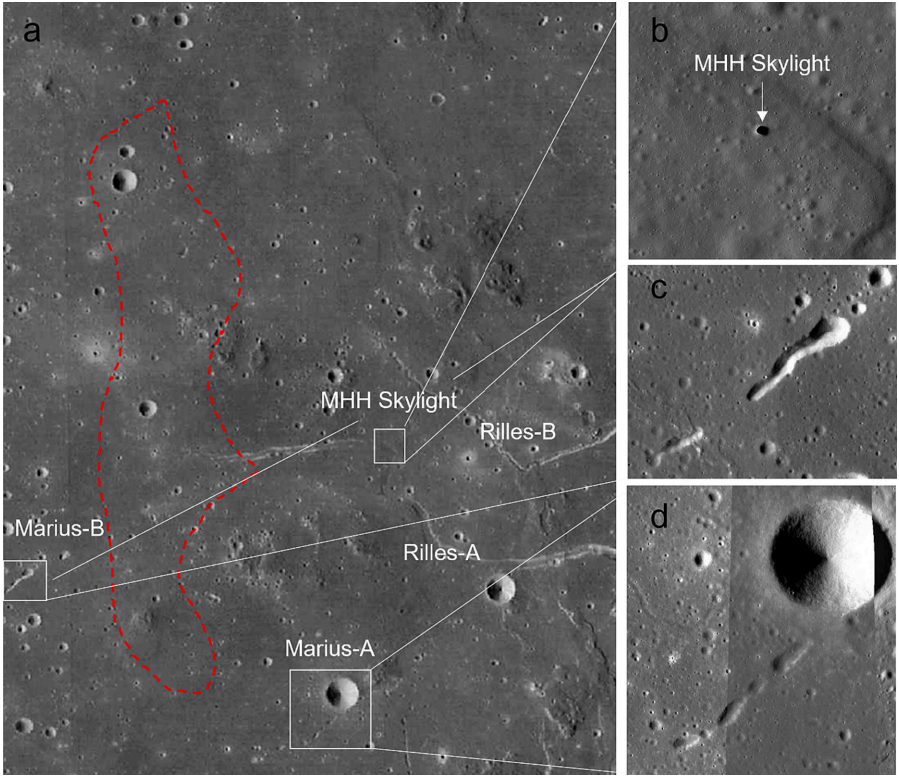
\includegraphics[width=0.66\linewidth]{marius_hills_collapse.png}
    \caption{LROC WAC image of the Marius Hills region, showing collapse chains, sinuous rilles, and skylights. The red dashed line marks the approximate path of the subsurface lava tube. 
    \textbf{(a)} Overview of the Marius Hills region with localized collapse chains and skylights. 
    \textbf{(b)} Close-up of the Marius Hills Hole (MHH). 
    \textbf{(c)} Marius-B collapse chain. 
    \textbf{(d)} Marius-A collapse chain. 
    Adapted from \citet{grails-gradients-mariushills}.}
    \label{fig:marius-hills-collapse}
\end{figure}

\subsection{Geophysical Evidence}

\textbf{Gravity Anomalies from GRAIL:} Subsurface cavities generate detectable gravitational anomalies, as the absence of mass in hollow voids results in a localized reduction in gravitational pull. Data from the \textbf{Gravity Recovery and Interior Laboratory (GRAIL)} mission has revealed mass deficits consistent with large voids beneath the surface at several lunar pit locations. The Marius Hills region provides a prominent example, where Bouguer gravity gradients identified a north-south anomaly linked to a subsurface lava tube. This anomaly was modeled as a hollow structure approximately 60 km long, 9 km wide, and 55 m high, buried at a depth of 605 m \citep{grails-gradients-mariushills} (see Figure \ref{fig:marius-hills-collapse}).

\textbf{Correlation with Surface Features:} The GRAIL mass deficit signature aligns with the position of known surface features, such as the Marius Hills skylight, further supporting the idea that the pit provides an access point to the underlying lava tube \citep{cavities-selene-lavatubes, grails-gradients-mariushills}. Additionally, similar gravity anomalies have been observed at other pit sites, lending credibility to the notion that subsurface voids are a common feature across multiple lunar regions \citep{cavities-selene-lavatubes, new-wagner}.

\begin{figure}[H]
    \centering
    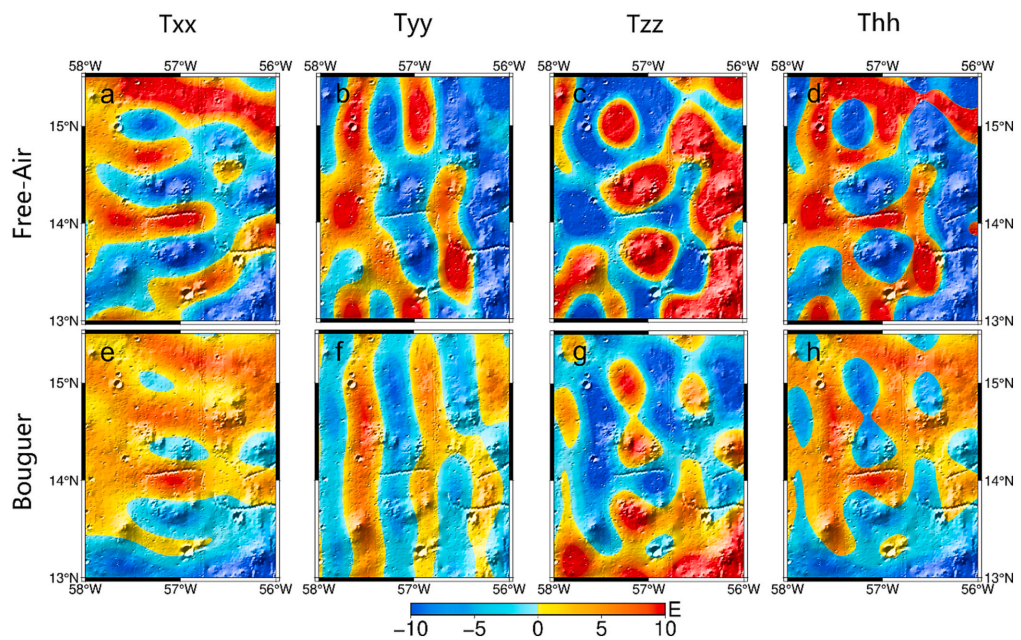
\includegraphics[width=0.85\linewidth]{grail-images-grabity.png}
    \caption{Gravity gradient observations at the Marius Hills region showing (top) Free-air gravity gradients \textbf{T$_{xx}$} (a), \textbf{T$_{yy}$} (b), \textbf{T$_{zz}$} (c), and \textbf{T$_{hh}$} (d); and (bottom) Bouguer gravity gradients \textbf{T$_{xx}$} (e), \textbf{T$_{yy}$} (f), \textbf{T$_{zz}$} (g), and \textbf{T$_{hh}$} (h). Cold colors (blue) indicate mass deficits, such as subsurface voids or valleys, while hot colors (red) correspond to mass surpluses, such as mounts or denser structures. The radial gradient \textbf{T$_{zz}$} highlights subsurface voids, whereas the horizontal components (\textbf{T$_{xx}$}, \textbf{T$_{yy}$}) reveal mass anomalies along the surface \cite{cavities-selene-lavatubes}.}
    \label{fig:marius-hills-gravity}
\end{figure}

\subsection{Radar Evidence}

\textbf{Radar Echoes from the Lunar Radar Sounder (LRS):} Radar sounders, such as the \textbf{Lunar Radar Sounder (LRS)} onboard the \textbf{SELENE (Kaguya)} spacecraft, have been instrumental in detecting intact subsurface voids. LRS data reveal distinctive radar reflection patterns, specifically a secondary radar echo following the initial surface reflection. This phenomenon, known as the “double-echo” signal, occurs when radar waves reflect off both the ceiling and floor of an underground cavity, indicating the presence of a void \citep{cavities-selene-lavatubes}.

At the Marius Hills region, LRS detected radar signals consistent with large, continuous underground voids. Similar findings have been confirmed by Carrer et al. (2024), who analyzed \textbf{Mini-RF radar} data of the Mare Tranquillitatis Pit (MTP). Their work demonstrated anomalous radar reflections beyond the pit walls, attributed to a subsurface cave conduit tens of meters long. This evidence supports the hypothesis that the MTP connects to an extensive underground lava tube, further reinforced by the alignment with other volcanic features and GRAIL gravity anomalies \citep{Carrer2024, cavities-selene-lavatubes}. These combined results highlight radar sounders as a critical tool for identifying accessible subsurface voids, corroborating morphological observations from LROC imagery.

\subsection{Thermal Evidence}

\textbf{Thermal Stability and Temperature Anomalies:} One of the most unique characteristics of lunar pits is their thermal environment. Surface temperatures on the Moon vary dramatically, from approximately 100 K during the lunar night to nearly 400 K in direct sunlight. However, thermal data from the \textbf{Diviner Lunar Radiometer} reveals that the interiors of pits maintain relatively stable temperatures. For instance, in the Mare Tranquillitatis pit, interior temperatures remain near -25°C throughout the lunar night \citep{thermal-lunar-pits}. 

This stability is explained by the concept of a \textbf{blackbody cavity}, where limited exposure to the lunar sky, combined with the insulating effects of the surrounding rock, creates a thermally stable environment. The overhanging walls and limited exposure to sunlight prevent excessive heating during the day, while the cavity retains thermal energy during the night. This thermal buffering effect is consistent with the behavior of sublunarean voids on Earth \citep{thermal-lunar-pits, newer-thermal}. 

\textbf{Potential for Volatile Trapping:} The thermal stability of lunar pits also supports the possibility of \textbf{volatile trapping}, particularly water ice, in shadowed regions of pit floors. Although lunar craters are known to act as cold traps where water ice accumulates, pits may offer similar advantages due to their shadowing geometry. Temperature models suggest that, under certain conditions, the interiors of pits remain cold enough to sustain water ice, especially in permanently shadowed areas \citep{newer-thermal, lunar-pits-numerical-modelling}. This capability is of particular interest for \textbf{in-situ resource utilization (ISRU)} efforts, as the ability to harvest water from lunar pits could provide a critical resource for human exploration and habitation \citep{newer-thermal}.

